\documentclass[a4paper, 12pt]{article}%тип документа

%отступы
\usepackage[left=2cm,right=2cm,top=2cm,bottom=3cm,bindingoffset=0cm]{geometry}

%Русский язык
\usepackage[T2A]{fontenc} %кодировка
\usepackage[utf8]{inputenc} %кодировка исходного кода
\usepackage[english,russian]{babel} %локализация и переносы

%Вставка картинок
\usepackage{wrapfig}
\usepackage{graphicx}
\usepackage{blindtext}
\graphicspath{{pictures/}}
\DeclareGraphicsExtensions{.pdf,.png,.jpg}

%оглавление
\usepackage{titlesec}
\titlespacing{\chapter}{0pt}{-30pt}{12pt}
\titlespacing{\section}{\parindent}{5mm}{5mm}
\titlespacing{\subsection}{\parindent}{5mm}{5mm}
\usepackage{setspace}

%Графики
\usepackage{multirow}
\usepackage{pgfplots}
\pgfplotsset{compat=1.9}

%Математика
\usepackage{amsmath, amsfonts, amssymb, amsthm, mathtools}

%Стиль страницы
\usepackage{fancyhdr}
\pagestyle{fancy}

\begin{document}

\begin{titlepage}

\begin{center}
%\vspace*{1cm}
\large\textbf{Московский Физико-Технический Институт}\\
\large\textbf{(государственный университет)}
\vfill
\line(1,0){430}\\[1mm]
\huge\textbf{Работа 4.7.3.}\\
\line(1,0){430}\\[1mm]
\vfill
\large Сибгатуллин Булат, ФРКТ\\
\end{center}

\end{titlepage}
\fancyhead[L] {Работа 4.7.3.}
\noindent \textbf{Цель работы:} \\
\indent ознакомление с методами получения и анализа поляризованного света.\\
\noindent \textbf{В работе используются:} \\
\indent оптическая скамья с осветителем; зелёный светофильтр; два поляроида; чёрное зеркало; полированная эбонитовая пластинка; стопа стеклянных пластинок; слюдяные пластинки разной толщины; пластинки в 1/4 и 1/2 длины волны; пластинка в одну длину волны для зелёного света (пластинка чувствительного оттенка).

\section*{Описание работы}

\section{Теоретическое введение}
	
	\subsection{Определение направления разрешённой плоскости колебаний поляроида}
	
	Определить направление разрешённых колебаний поляроида проще всего с помощью чёрного зеркала.
	
При падении света на отражающую поверхность под углом Брюстера, свет в отражённом луче почти полностью поляризован, а вектор E
параллелен отражающей поверхности ("<правило иголки">). Луч света,
прошедший поляроид и отразившийся от чёрного зеркала, имеет минимальную интенсивность при выполнении двух условий: во-первых, свет
падает на отражающую поверхность под углом Брюстера и, во-вторых,
в падающем пучке вектор E лежит в плоскости падения.

Вращая поляроид вокруг направления луча и чёрное зеркало вокруг
оси, перпендикулярной лучу, методом последовательных приближений
можно добиться минимальной яркости луча, отражённого от зеркала,
и таким образом определить разрешённое направление поляроида.

Измеряя угол поворота зеркала (угол Брюстера), нетрудно определить коэффициент преломления материала, из которого изготовлено
зеркало. Описанный метод часто используется для измерения коэффициента преломления непрозрачных диэлектриков.

\subsection{Получение эллиптически поляризованного света}
\begin{wrapfigure}{r}{0.35\linewidth} 
	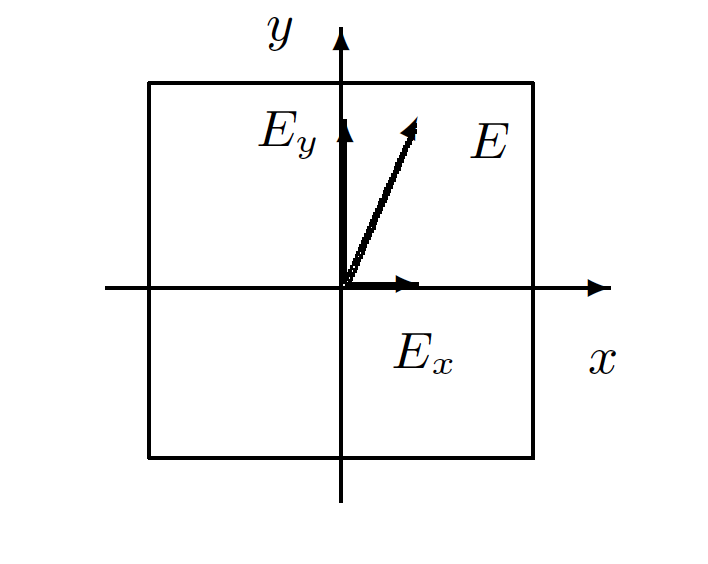
\includegraphics[width=\linewidth]{images/1.png}
	\caption{Разложение линейно поляризованного света по главным направлениям двоякопреломляющей пластинки}
	\label{ris 1}
\end{wrapfigure}

Эллиптически поляризованный свет можно получить из линейно поляризованного с
помощью двоякопреломляющих кристаллических пластинок.

Двоякопреломляющая пластинка имеет два взаимно перпендикулярных главных направления, совпадающих с осями эллипсоида диэлектрической проницаемости. Волны, поляризованные вдоль главных направлений, распространяются в пластинке с разными скоростями, не изменяя характера своей поляризации. Эти волны называются главными. Мы будем обозначать показатели преломления для главных волн через $ n_x $ и $ n_y $, где $ x $ и $ y $ --- главные направления кристаллической пластинки (рис. 1).

Пусть на пластинку падает линейно поляризованная волна, электрический вектор которой ориентирован под некоторым углом $ \alpha $ к оси
$ x $. Разложим вектор $ \mathbf{E} $ на составляющие $ E_x $ и $ E_y $. На входе пластинки $ E_x $ и $ E_y $ находятся в фазе. На выходе из-за разности скоростей между ними появляется разность хода $ d(n_x - n_y) $, при этом сдвиг фаз определяется соотношением

\begin{equation}\label{}
\Delta \phi =  \dfrac{2\pi}{m} = k d(n_x - n_y)
\end{equation}
Как уже отмечалось, при сложении двух взаимно перпендикулярных колебаний, обладающих некоторым сдвигом фаз, образуется колебание, поляризованное по эллипсу.

\begin{wrapfigure}{l}{0.35\linewidth}
	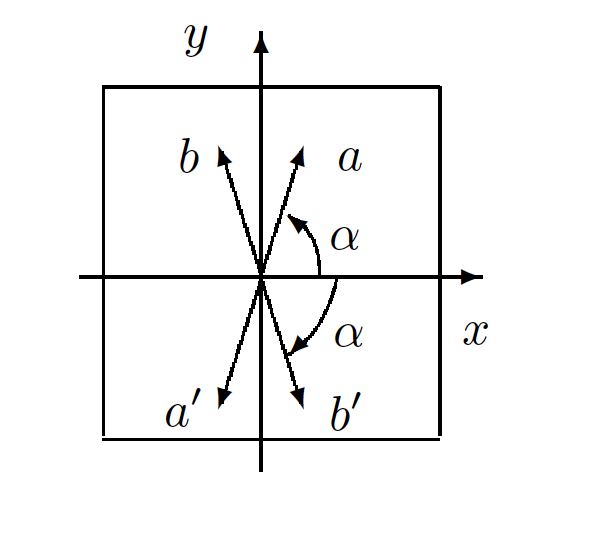
\includegraphics[width=\linewidth]{images/2.png}
	\caption{Поворот направления колебаний с помощью пластинки в $ \lambda / 2 $}
	\label{ris 2}
\end{wrapfigure}


Рассмотрим практически важные частные случаи.

 \begin{enumerate}
 		
 	\item Пластинка даёт сдвиг фаз $ 2\pi $ (пластинка в длину волны $ \lambda $). В результате сложения волн на выходе пластинки образует-
ся линейно поляризованная волна с тем же направлением колебаний, что и в падающей волне.

	\item Пластинка даёт сдвиг фаз $ \pi $ (пластинка в полдлины волны $ \lambda / 2 $). На выходе пластинки снова образуется линейно поляризованная волна. Направление $ bb' $ колебаний этой волны повёрнуто относительно направления $ aa' $ колебаний падающей волны (рис. 2). Как нетрудно сообразить, направление $ bb' $ является зеркальным отображением направления $ aa' $ относительно одного из главных направлений пластинки. Такую пластинку используют для поворота направления колебаний линейно поляризованного света.
	
	\item Пластинка создаёт между колебаниями сдвиг фаз $ \pi/2 $ (пластинка
в четверть длины волны). При сложении двух взаимно перпендикулярных колебаний, имеющих разность фаз $ \pi/2 $, образуется эллипс, главные оси которого совпадают с координатными осями $ x $ и $ y $. При равенстве амплитуд возникает круговая поляризация.
 	
 \end{enumerate}

Следует отметить, что, говоря о пластинках $ \lambda , \lambda/2, \lambda/4  $ и т. д., всегда подразумевают какую-либо вполне определённую монохроматическую
компоненту (например, пластинка $ \lambda/2 $ для зелёного света). Если на двоякопреломляющую пластинку падает не монохроматический свет, то на
выходе из неё для разных спектральных компонент эллипсы поляризации будут различными.

\subsection{Анализ эллиптически поляризованного света}

Анализ эллиптически поляризованного света сводится к нахождению главных осей
эллипса поляризации и к определению направления вращения электрического вектора.

Главные оси эллипса поляризации определяются с помощью анализатора по максимуму и минимуму интенсивности проходящего света.
Направление вращения электрического вектора может быть найдено
с помощью пластинки в четверть длины волны, для которой известно,
какая из главных волн, $ E_x $ или $ E_y $, имеет б\'{o}льшую скорость распространения (и соответственно меньшее значение показателя преломления).

Выберем для определённости координатные оси x и y на пластинке
так, чтобы $ nx < ny $. В этом случае главная волна $ E_x $ имеет большую
скорость распространения. Поместим такую пластинку на пути эллиптически поляризованного света и совместим главные направления пластинки $ \lambda/4 $ с главными осями эллипса поляризации. На выходе из этой
пластинки сдвиг фаз между $ E_x $ и $ E_y $ вместо $ \pi/2 $ станет равным ну-
лю или $ \pi $. Свет окажется линейно поляризованным. Из двух возможных значений сдвига фаз, 0 или $ \pi $, реализуется одно: то, которое соответствует имеющемуся в волне направлению вращения электрического вектора.

Рассмотрим, например, случай, когда электрический вектор в эллиптически поляризованной волне вращается против часовой стрелки,
если смотреть навстречу лучу. В этом случае, очевидно, в волне, падающей на пластинку в $ \lambda/4 $, колебание $ E_y $ отстаёт по фазе на $ \pi/2 $ от
колебания $ E_x $. При прохождении через пластинку разность фаз увеличивается до $ \pi $. Таким образом на выходе из пластинки возникают линейно поляризованные волны со сдвигом фаз $ \pi $. Сложение этих волн
даёт плоскополяризованную волну, электрический вектор которой рас-
полагается во втором и четвёртом квадрантах координатной системы
$ x, y $.

Рассуждая аналогичным образом, найдём, что при вращении электрического вектора по часовой стрелке направление колебаний в линейно поляризованной волне, выходящей из пластинки, располагается в первом и третьем квадрантах. Определяя направление колебаний на выходе из пластинки с помощью поляроида, можно, таким образом, определить характер эллиптической поляризации (вращение против или по часовой стрелке).

\subsection{Пластинка чувствительного оттенка}

\begin{wrapfigure}{l}{0.35\linewidth}
	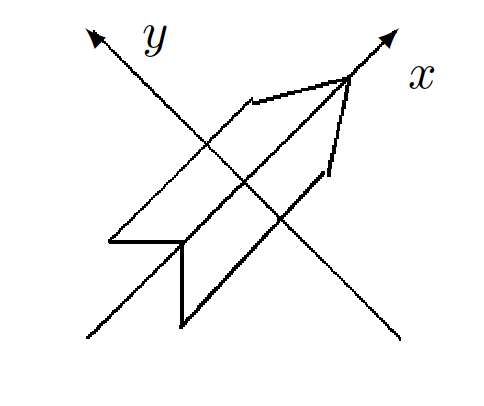
\includegraphics[width=\linewidth]{images/3.png}
	\caption{Пластинка
чувствительного
оттенка}
	\label{ris 3}
\end{wrapfigure}

Выше предполагалось известным, какому из двух главных направлений пластинки в четверть длины волны соответствует большая скорость распространения света.
Установить это можно различными способами, например с помощью
пластинки чувствительного оттенка (так называют пластинку в $ \lambda $
для зелёной спектральной компоненты, $ \lambda = 560 $ нм).

Пластинка имеет форму стрелы (рис. 3), вдоль оси которой расположено главное направление, соответствующее большей скорости распространения.

Если пластинка чувствительного оттенка помещена между скрещенными поляроидами и главные направления пластинки не параллельны
направлениям разрешённых колебаний поляроидов, то при освещении
белым светом пластинка кажется окрашенной в лилово-красный цвет.
Это объясняется тем, что зелёная компонента линейно поляризованного света при прохождении пластинки не меняет поляризации и задерживается вторым поляроидом. Для красной и фиолетовой компонент
пластинка создаёт сдвиг фаз, несколько отличный от $ 2\pi $. На выходе
из пластинки красная и фиолетовая компоненты оказываются поэтому
эллиптически поляризованными и частично проходят через второй поляроид. Таким образом, в известном смысле наблюдаемый в указанном
опыте цвет пластинки дополнителен к зелёному.

Если между скрещенными поляроидами поместить пластинку чувствительного оттенка
($ \lambda $) и пластинку в $ \lambda/4 $ так, чтобы их главные
направления совпадали, цвет пластинки изменится. Если у пластинки чувствительного оттенка и пластинки в $ \lambda/4  $совпадут главные направления, соответствующие большей скорости распространения, то разность хода между $ E_x $ и $ E_y $ для зелёного света составит уже $ 5\lambda/4 $. Это соответствует разности хода в $ \lambda $ для света с большей длиной волны, т. е. для "<более красного"> света. При освещении
этих пластинок (напомним, что они расположены между скрещенными поляроидами) белым светом теперь погасится не зелёная, а красная
часть спектра, и проходящий свет будет казаться зеленовато-голубым.
Если же главные направления, соответствующие большей скорости распространения, у пластинки чувствительного оттенка и у пластинки
в $ \lambda/4 $ окажутся перпендикулярными, то проходящий свет приобретёт
оранжево-желтую окраску (погасится фиолетово-голубая часть спектра).

Изменение цвета позволяет, таким образом, определить, какое из
главных направлений пластинки в $ \lambda/4 $ соответствует большей скорости
распространения.

\subsection{Интерференция поляризованных лучей}

\begin{wrapfigure}{r}{0.35\linewidth}
	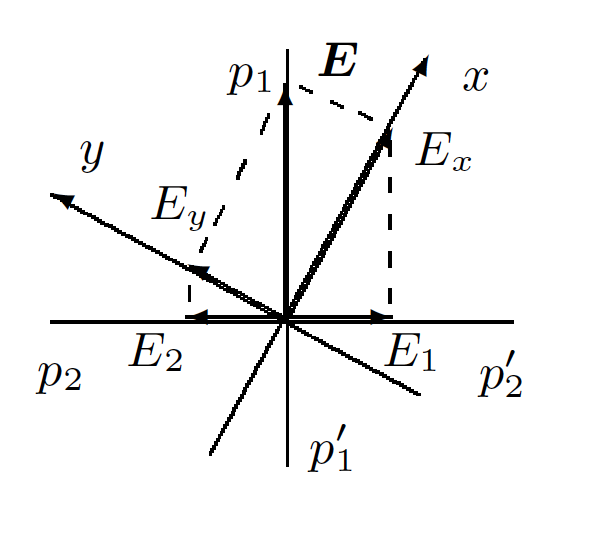
\includegraphics[width=\linewidth]{images/4.png}
	\caption{К объяснению интерференции
поляризованных лучей}
	\label{ris 4}
\end{wrapfigure}


Тонкие двоякопреломляющие пластинки, помещённые между поляроидами, кажутся окрашенными. Эта окраска может быть истолкована как результат интерференции поляризованных лучей. На рис. 4 представлена схема для
случая скрещенных поляроидов.

Здесь $ p1p'1 $ --- разрешённое направление колебаний поляризатора
(первого поляроида); $ x, y $ --- координатная система, связанная с главны-
ми направлениями двоякопреломляющей пластинки; $ p2p'2 $ --- разрешённое направление колебаний анализатора (второго поляроида). Волны
$ E_x  $ и $ E_y $ на выходе из пластинки когерентны, но не могут интерферировать, так как $ E_x \perp  E_y $. Волны $ E_1 $ и $ E_2 $ на выходе второго поляроида
также являются когерентными и к тому же поляризованы в одной плоскости. Эти волны интерферируют между собой. Результат интерференции определяется зависящим от длины волны сдвигом фаз между $ E_1 $
и $ E_2 $. В результате интерференции поляризованных лучей пластинка, освещаемая белым светом, кажется окрашенной.

Если поворачивать двоякопреломляющую пластинку, расположенную между
скрещенными поляроидами, то соотношение амплитуд волн $ E_1 $ и $ E_2 $ и разность фаз между ними не изменяются. Это означает, что цвет пластинки при её поворотах не меняется, а меняется только интенсивность света. За один оборот пластинки интенсивность четыре раза обращается в нуль --- это происходит при совпадении главных направлений
$ x $ и $ y $ с разрешёнными направлениями колебаний поляроидов.

Если же двоякопреломляющую пластинку оставить неподвижной, а
второй поляроид повернуть так, чтобы разрешённые направления $ p1p'1 $
и $ p2p'2 $ совпали, то волны $ E_1 $ и $ E_2 $ приобретают дополнительный фазовый сдвиг на $ \pi $ для всех спектральных компонент; при этом их амплитуды изменятся так, что цвет пластинки изменится на дополнительный. 

\section{Ход работы}

\begin{enumerate}

\item Разместим на оптической скамье осветитель S, поляроид $P_1$ и черное зеркало (пластинку черного стекла) так, чтобы плоскость падения была горизонтальна. Свет, отраженный от зеркала, рассматриваем сбоку, расположив глазз таким образом, чтобы вблизи оси вращения зеркала можно было увидеть изображение диафрагмы осветителя. Поворачивая подляроид в этом положении и вращением зеркала вокруг вертикальной оси снова добьемся минимальной интенсивности отраженного луча.

Для первого поляроида разрешенное направление горизонтальное, на лимбе $231^{\circ}$.

Вместо черного зеркала поставим второй поляроид. Скрестим их, определим разрешенное направление второго поляроида -- горизонтальная волна, на лимбе $128^{\circ}$.

\item Поставим на скамью эбонитовую пластину с круговой пластиной.

Повернем эбонитовое зеркало вокруг вертикальной оси так, чтобы его плоскость была перпендикулярна лучу и попытаемся совместить отраженное от эбонита пятно с отверстием осветителя.

Установим направление разрешенных колебаний поляроида $P_1$ горизонтально и найдем угол поворота эбонита, при котором интенсивность отраженного луча минимальна: $\varphi_b = 58^{\circ}.$

Повторим измерения добавив светофильтр Ф и сравним результаты - они получились одинаковыми.

По углу Брюстера рассчитаем показатель преломления эбонита и сравним с табличным:

\[n = \tan (\varphi) = 1,598,\]

здесь табличное значение равно $n = 1,6$.

\item Поставим стопу стеклянных пластинок вместо эбонитового зеркала и подберем для неё такое положение, при котором свет падает на стопу под углом Брюстера. Осветим стопу неполяризованным светом (снимем поляризатор с оптической скамьи) и, рассматривая через поляроиды свет, отраженный от стопы, определим ориентацию ветора \textbf{E} в отраженном луче и характер поляризации света в преломленном луче - наблюдая прошедший через стопу свет. Запишем полученные углы: для $P_1 = 221^{\circ}$, для $P_2 = 128^{\circ}$.

\begin{figure}[h!]
\centering
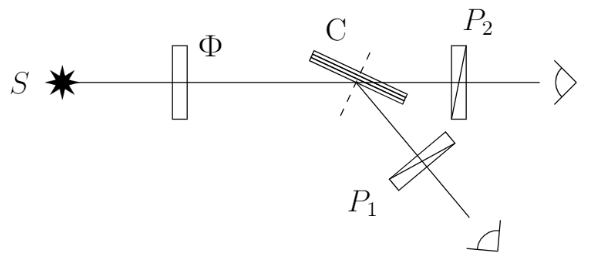
\includegraphics[scale=1]{images/mirror.png}
\caption{Исследование стопы}
\label{mirror}
\end{figure}

$P_1 - P_2 = 93^{\circ}$ (убеждаемся, что поляризации отраженного и преломленного луча света). Преломленные лучи горизонтальные, отраженные - вертикальные. Установили, что лучи имеют правый круговой тип поляризации.

\item Поставим кристаллическую пластинку между скрещенными поляроидами $P_1$ и $P_2$. Вращая пластинку вокруг направления луча и наблюдая за интенсивностью света проходящего сквозь второй поляроид, определим, при каком условии главные направления пластинки совпадают с разрешенными направлениями поляроидов. Повторим опят для второй пластинки.

\begin{figure}[h!]
\centering
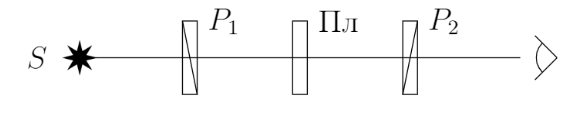
\includegraphics[scale=1]{images/main.png}
\caption{Определение главных плоскостей двоякопреломляющих пластин}
\label{main}
\end{figure}

\begin{center}
\begin{tabular}{|c|c|}
\hline 
Пластинка 1 & Пластинка 2 \\ 
\hline 
min, $^{\circ}$: 8; 278& min, $^{\circ}$: 324; 233\\ 
\hline 
max, $^{\circ}$: 320; 234& max, $^{\circ}$: 275; 190\\ 
\hline 
\end{tabular} 
\end{center}

Минимумы и максимумы интенсивности чередуются через $45^{\circ}$, главные плоскости пластин совпадают с разрешенными направлениями поляроидов при максимальной интенсивности.

\item Добавим в схеме зеленый фильтр: установим разрешенное направление поляроида, а главные направления исследуемой пластинки под углом $45^{\circ}$ к горизонтали.

Пластинка $\lambda/ 2$ не изменяет характер поляризации, при ее повороте меняется интенсивность, а поляризация остается линейной.

Пластинка $\lambda/ 4$ создается сдвиг фаз $\pi / 2$ между колебаниями -- элллиптическая поляризация. Эта пластинка не меняет интенсивность при повороте.

\item Поставим между скрещенными поляроидами пластинку чувствительного оттенка (для зелёного света), имеющую вид стрелки. Световой вектор, ориентированный вдоль направления стрелки, проходит с большей скоростью, перпендикулярный с меньшей.
		
Установили разрешённое направление первого поляроида горизонтально и убедились с помощью второго поляроида, что эта пластинка не меняет поляризацию зелёного света в условиях предыдущего опыта.
		
Убрали зелёный фильтр и поставили между скрещенными поляроидами пластинку $\lambda$ (стрелка под углом $45^\circ$ к разрешённым направлениям поляроидов). Глядя сквозь второй поляроид на стрелку, убудились, что она имеет пурпурный цвет. Это связано с тем, что зелёный свет задерживается вторым поляроидом, а красная и синяя компоненты проходят.

\begin{figure}[h!]
\centering
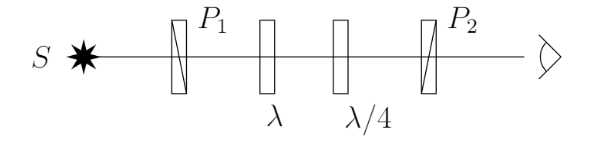
\includegraphics[scale=1]{images/speed.png}
\caption{Определение направлений большей и меньшей скорости}
\label{speed}
\end{figure}
		
Добавили к схеме пластинку $\lambda/4$, главные направления которой совпадают с главными направлениями пластины $\lambda$ и ориентированы под углом $45^\circ$ к разрешённым направлениям скрещенных поляроидов. При повороте рейтера со стрелкой на $180^\circ$ вокруг вертикальной оси цвет стрелки меняется от зелёно-голубого до оранжево-жёлтого. При совпадении быстрой оси стрелки и главного направления пластинки суммарная разность хода для зеленого света составит $5\lambda/4$, что приблизительно равно длине волны в красном спектре, поэтому красный свет будет задерживаться поляроидами, что объясняет зелёно-голубой цвет стрелки. При совпадении медленой оси с главным направлением пластинки разность хода $3\lambda /4$ будет составлять длину волны для фиолетово-голубой части спектра, поэтому в результате увидим оранжево-жёлтый цвет.
		
\item Нарисовали эллипс поляризации для вектора	$\vec{E}$, вышедшего из пластинки $\lambda/4$, где большей скорости соответствует ось $x$, а также две вышедших из пластинки синусоиды: $x(t)$ и $y(t)$ со сдвигом фаз в четверть периода. Проанализировали графики и определили направление вращения электрического вектора в эллиптически поляризованной волне. 

\begin{figure}[h!]
\centering
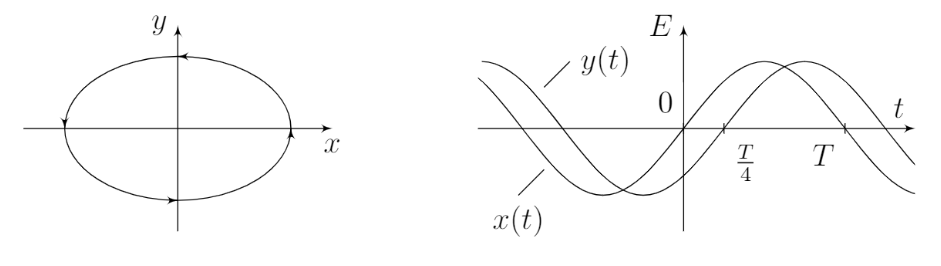
\includegraphics[scale=1]{images/pol_ellips.png}
\caption{Эллипс поляризации и две синусоиды}
\label{pol_ellips}
\end{figure}

Снова поставили зелёный фильтр, а за ним между скрещенными поляроидами --- пластинку произвольной толщины.

Получили эллиптически-поляризованный свет. Для этого установили разрешённое направление первого поляроида под углом 10–20$^\circ$ к горизонтали так, чтобы вектор $\vec{E}$ падающего на пластинку света был расположен в первом квадранте. Установили разрешённое направление второго поляроида вертикально и, вращая пластинку, нашли минимальную интенсивность света, прошедшего второй поляроид. Вращая второй поляроид, убедились, что свет поляризован эллиптически, а не линейно. Таким образом получили эллипс поляризации с вертикально ориентированной малой осью.

Для определения направления вращения светового вектора в эллипсе установили между поляроидами дополнительную пластинку $\lambda/4$ с известными направлениями «быстрой» и «медленной» осей, ориентированными по осям эллипса поляризации анализируемого света. В этом случае вектор $\vec{E}$ на выходе такой, как если бы свет прошёл две пластинки $\lambda/4$: свет на выходе из второй пластинки будет линейно поляризован. Если пластинки поодиночке дают эллипсы, вращающиеся в разные стороны, то поставленные друг за другом, они скомпенсируют разность фаз, и вектор $\vec{E}$ на выходе останется в первом и третьем квадрантах. Если же световой вектор перешёл в смежные квадранты, значит, эллипсы вращаются в одну сторону. А как вращается эллипс в пластинке $\lambda/4$, определили раньше.
	
\item Расположили между скрещенными поляроидами мозаичную слюдяную 	пластинку. Она собрана из 4-х узких полосок слюды, лежащих по сторонам квадрата (две полоски «толщиной» $\lambda/4$ и по одной --- $\lambda/2$ и $3\lambda/4$). В центральном квадратике слюды нет. Главные направления всех пластинок ориентированы параллельно сторонам квадрата. Вращая пластинку, наблюдали изменения (цвета или интенсивности) в отдельном квадратике. Потом, не трогая пластинки, вращали второй поляроид. Наблюдаемые эффекты:

Вращаем пластинку: изменяется интенсивность света с периодичностью $\pi/4$;

Вращаем второй поляроид: изменяется (инверсируется) цвет пластинок также с периодичностью  $\pi/4$.
		    
\begin{figure}[h!]
        \begin{center}
            \begin{minipage}[h!]{0.48\linewidth}
                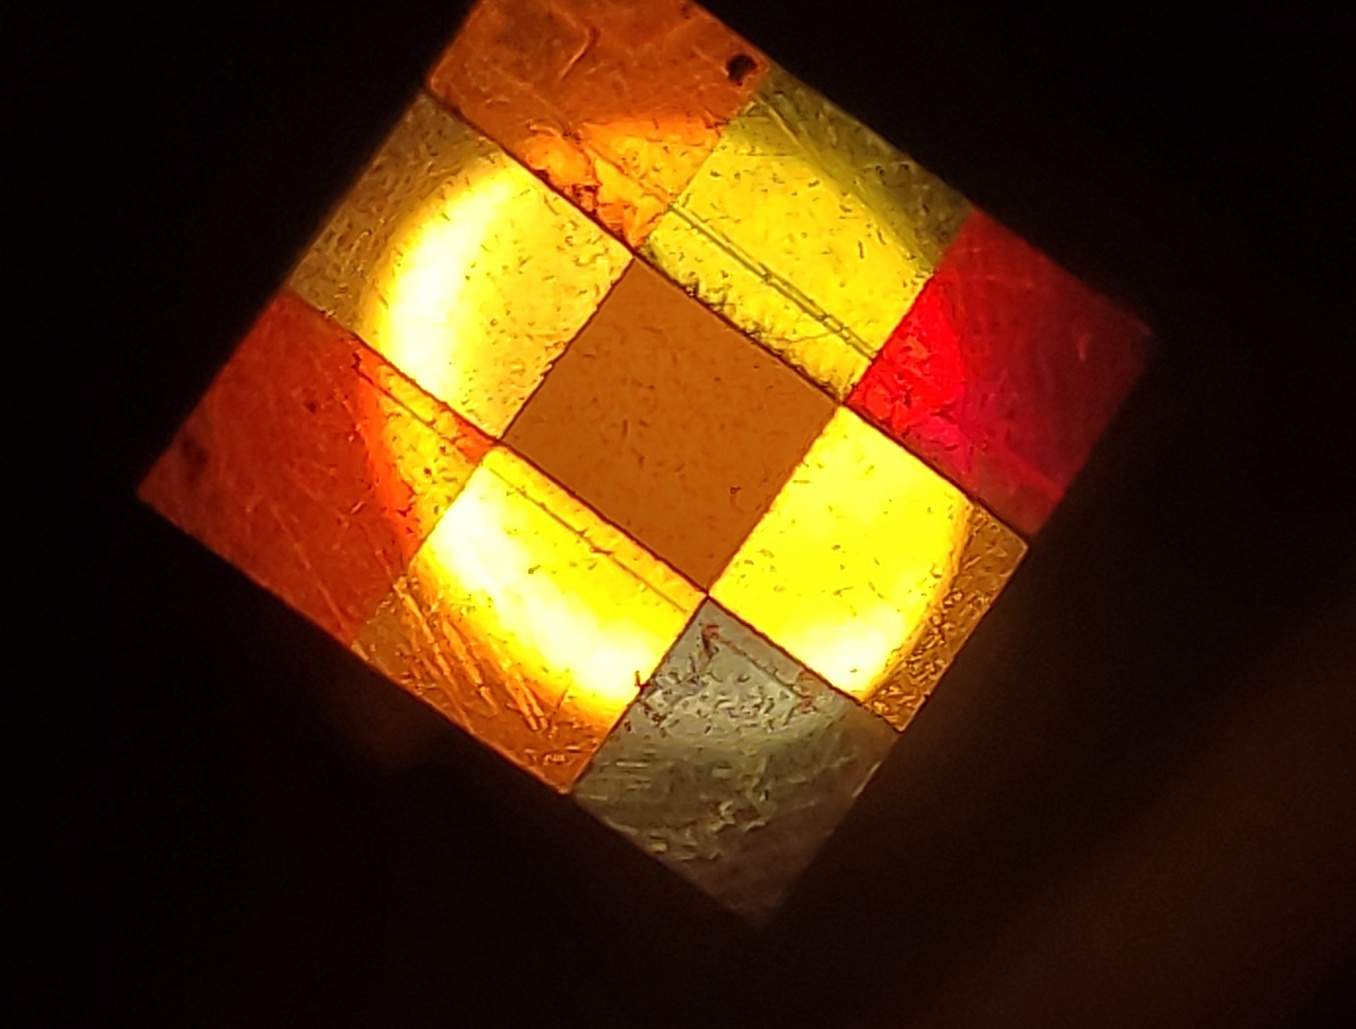
\includegraphics[width=1\linewidth]{images/stopa_1.jpg}
                \caption{Картина цветов пластинок в стопе (1)}
                \label{picture_2}
            \end{minipage}
            \hfill
            \begin{minipage}[h!]{0.48\linewidth}
                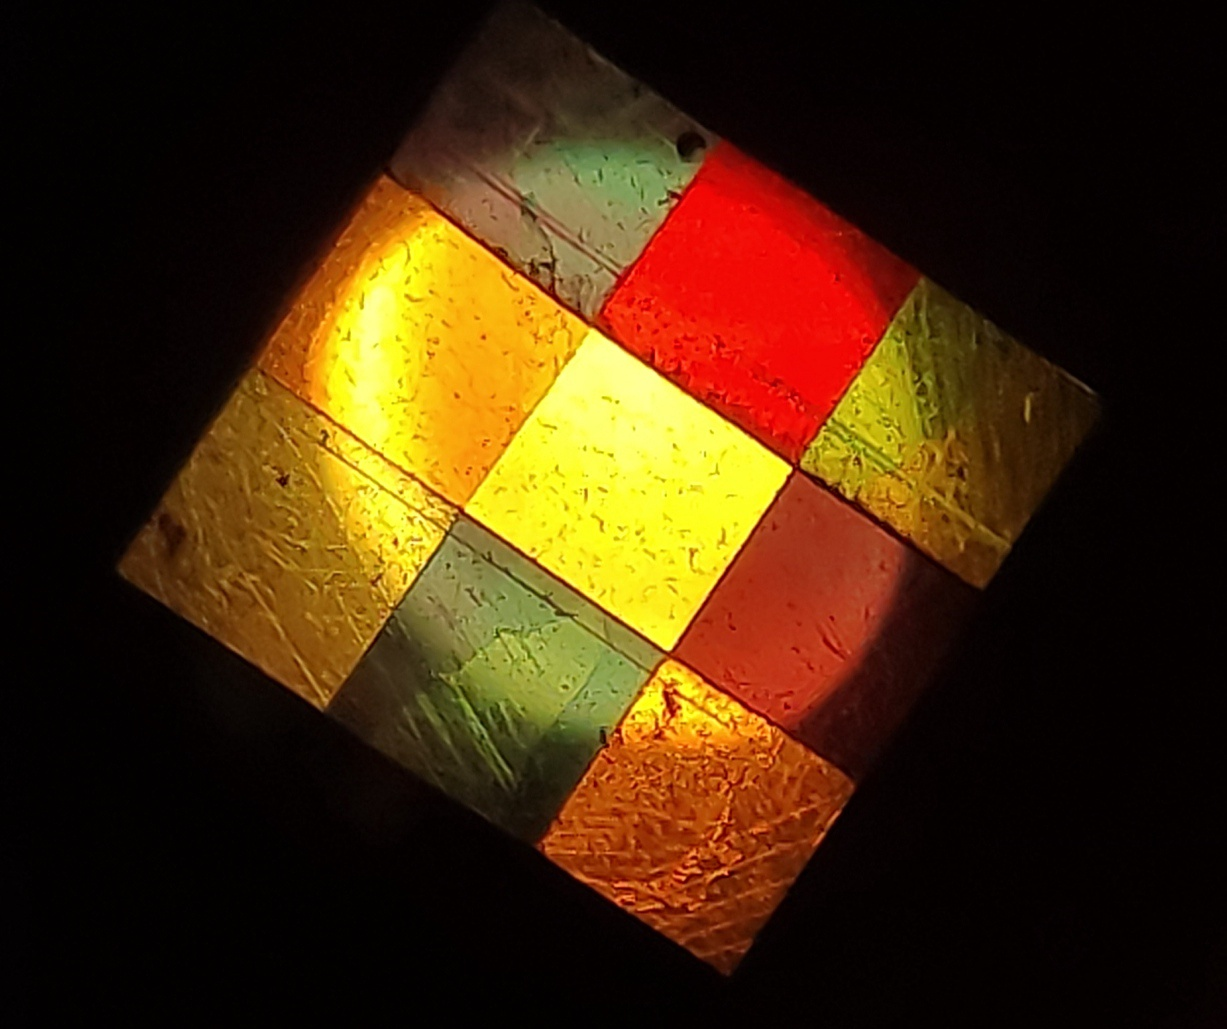
\includegraphics[width=1\linewidth]{images/stopa_2.jpg}
                \caption{Картина цветов пластинок в стопе (2)}
                \label{picture_3}
            \end{minipage}
        \end{center}
    \end{figure}

\end{enumerate}

\section*{Вывод}
Изучили явления связанные с поляризацией света: определили разрешённые направления поляроидов и с помощью них проводили следующие опыты. Рассмотрели угол Брюстера, с помощью него определили показатель преломления эбонита. Для двоякопреломляющих пластин определили главные направления, а так же тип пластинок --- $\lambda /4$ и $\lambda/2$. Также исследовали пластинку чувствительного оттенка, определили быструю и медленную оси и рассмотрели эффекты, происходящие при прохождении света через комбинацию пластинок. Получили эллиптически поляризованную волну, рассмотрели интерференцию поляризованных лучей в мозаичной слюдяной пластинке.


\end{document}